\documentclass{NSF}
\usepackage{amssymb}
\usepackage{amsmath}
\usepackage{amsthm}
\usepackage{graphicx}
\usepackage[table,xcdraw]{xcolor}
\usepackage{pgf,tikz,pgfplots,tikzscale}
\pgfplotsset{compat=1.14}
\usepackage{mathrsfs}
\usetikzlibrary{arrows}
\usepackage{subfig}
\graphicspath{ {images/} }

% https://www.overleaf.com/learn/latex/Theorems_and_proofs
\newtheorem{theorem}{Theorem}[section]
\newtheorem{corollary}{Corollary}[theorem]
\newtheorem{lemma}[theorem]{Lemma}



\begin{document}
\title{{\normalfont Computer Science Capstone Final Report}\\Lifting Squares to a Half-space: a Specific Case of Lifting Pseudo-disks}
\author{Myunggun Seo,  Guyu Fan, and Nischal Mainali \\ Professor: Saurabh Ray}
\date{May 15, 2019}


{\let\newpage\relax\maketitle}

\section{Abstract}
% Your short version of your proposal goes here
A half-space in $\mathbb{R}^3$ is either of the two parts separated by a plane. Because of some helpful properties that exist in half-spaces, it is often useful to map geometries in a plane to half-spaces in  $\mathbb{R}^3$. In this project, we attempt to prove or disprove the existence of a mapping from a family of squares in a plane to a family of half-spaces in $\mathbb{R}^3$ such that all points inside each square are mapped to points inside the corresponding half-space and all points outside each square are mapped to points outside the corresponding half-space. If such a mapping can be shown to exist, we attempt to provide a mathematical description of it or find an algorithm that performs the mapping.

\newpage
\tableofcontents

\newpage
\section{Introduction}
\subsection{General Case of Lifting Pseudo-disks}
The problem that we tackle is a specific case of an unsolved problem in computational geometry: 

Given a set of pseudo-disks $\{D_i\}$ and points $\{P_j\}$ in $\mathbb{R}^2$ in arbitrary positions, (1) determine the existence of a mapping and (2) describe the mapping from the pseudo-disks and points to a set of half-spaces $\{H_i\}$ and points $\{Q_j\}$ in $\mathbb{R}^3$ such that the membership of point $P_j$ in a pseudo-disk $D_i$ is preserved with point $Q_j$ in $H_i$. 

Because shapes in $\mathbb{R}^2$ are mapped to a higher dimension $\mathbb{R}^3$, we will call this problem ``lifting." Note that this mapping is injective but need not be surjective. Also, no point in the half-space is lifted from the exterior of the pseudo-disk.

Lifting is part of a class of mapping methods in Combinatorial Geometry which proved useful because such maps provide another representation and thus new properties to a geometric configuration. Such new properties are often used in cases such as finding lower bounds on $\epsilon$-nets or in Kernel Trick in Machine Learning. 

For circles, this mapping exists and can be described algebraically, but it is not known whether there is such a mapping for other seemingly simple cases like ellipses, rectangles, or squares. 

\subsection{Case of Squares of Equal Size}
Problem statement: Given a set of squares of  $\{S_i\}$ and points $\{P_j\}$ in $\mathbb{R}^2$ in arbitrary positions, is there a mapping from the squares and points to a set of half-spaces $\{H_i\}$ and points $\{Q_j\}$ in $R^3$ such that the membership of point $P_j$ in a square $S_i$ is preserved with point $Q_j$ in $H_i$? If there is, what is the mapping? 

\section{Problems Related to Pseudo-disk Lifting Problem}
\subsection{Solution: Lifting an interval}
This is the lowest abstraction of a pseudo-disk that we consider. An interval in $\mathbb{R}$ can be considered both as a circle (or ball) and a square (or $k$-cell). The interval, using the definition of a ball, defined as $|x-a|\leq r$ is equivalent to $(x-a)^2 \leq r^2$ and $x^2-r^2$ is substituted with $y$ to construct the half-space in $\mathbb{R}^2$: $-2ax+y+a^2 \leq 0$.  Point $x=\alpha$ is lifted to $(\alpha, \alpha^2)$. Then all points inside the original interval of length $2r$ becomes placed below the $\mathbb{R}^2$ hyperplane, which is a line.
\begin{align*}
\alpha & \mapsto (\alpha,\alpha^2) \\
|x-a|\leq r & \mapsto -2ax + y + a^2 \leq 0
\end{align*}


\subsection{Solution: Lifting disks of equal radii}
\begin{figure}[ht]
\centering
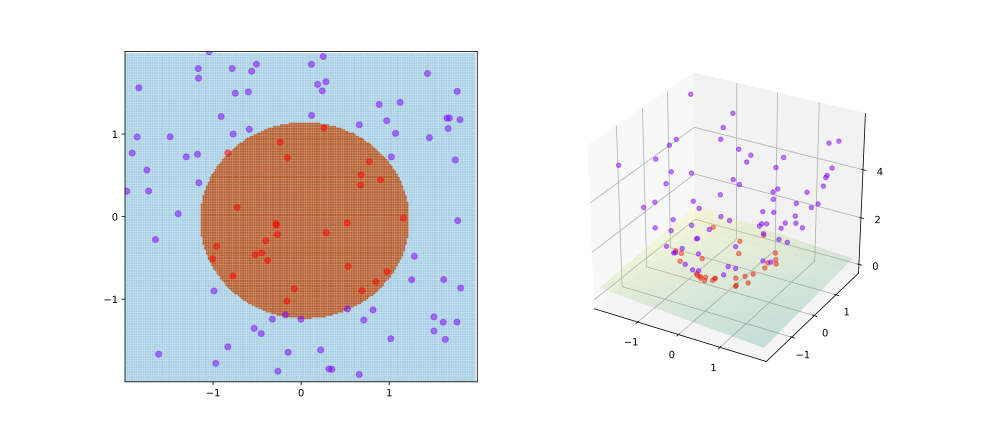
\includegraphics[width=\textwidth]{images/kernel-trick}
\caption{Red points inside a single disk in $\mathbb{R}^2$ are mapped to a half-space in $\mathbb{R}^3$, allowing linear separation of points.  (Image Source: Wikipedia - Kernel Method) }
\end{figure}

There is an algebraic lifting from disks to half-spaces. Point $(\alpha,\beta)$ is lifted to $(\alpha,\beta,\alpha^2+\beta^2-r^2)$, and disk $(x-a)^2+(y-b)^2\leq r^2$ is lifted to $-2ax -2by + z + (a^2+b^2) \leq 0$ by substituting  $x^2+y^2-r^2$ with $z$. 
\begin{align*}
(\alpha,\beta) & \mapsto (\alpha,\beta,\alpha^2+\beta^2-r^2) \\
(x-a)^2+(y-b)^2\leq r^2 & \mapsto -2ax -2by + z + (a^2+b^2) \leq 0
\end{align*}

The limitation of this method is that it is only possible for disks of equal radii since all points in $\mathbb{R}^2$ can only map to the same point in $\mathbb{R}^3$ which will be defined by the radius $r$.

\subsection{Solution: Lifting disks of varying radii}
\label{section:disk-lifting}
Using a similar approach as the above, Point $(\alpha,\beta)$ is lifted to $(\alpha,\beta,\alpha^2+\beta^2)$, and disk $(x-a)^2+(y-b)^2\leq r^2$ is lifted to $-2ax -2by + z + (a^2+b^2-r^2) \leq 0$ by substituting  $x^2+y^2$ with $z$. 
\begin{align*}
(\alpha,\beta) & \mapsto (\alpha,\beta,\alpha^2+\beta^2) \\
(x-a)^2+(y-b)^2\leq r^2 & \mapsto -2ax -2by + z + (a^2+b^2-r^2) \leq 0
\end{align*}

\subsection{Idea: Straightening pseudo-disks to disks}
If there is a way to ``straighten," or map, a set of pseudo-disks to disks, then there must be a way to lift any pseudo-disk to a half-space by straightening the pseudo-disks to disks and lifting the produced disks. There exist some topologies of pseudo-disks that cannot expressed using disks. However, as long as pre-existing regions are preserved, we allow new regions to exist.

\begin{figure}[ht]
\centering
\subfloat[]{\includegraphics[width = 0.4\textwidth]{topologically-impossible-ellipse}}
\subfloat[]{\includegraphics[width = 0.4\textwidth]{topologically-impossible-circle}} 
\caption{An example of straightening of pseudo-disks. Injective but not neccessarily surjective mappings are of interest to us. Some new regions may exist other than the image.}
\label{fig:topologically-impossible}
\end{figure}

\subsection{Idea: Straightening pseudo-lines to lines}
A similar problem to straightening pseudo-disks to disks is straightening pseudo-lines. Pseudo-lines are a set of curves that intersect one another at most once. This property derives from that of lines. The problem statement is:  given a set of $n$ pseudo-lines, find a positioning of $n$ lines so that the vertical order of the lines match that of the pseudo-lines.



\subsection{Idea: Lifting pseudo-disks to a polytope}
A pseudo-disk can be considered as an (infinite) intersection and complements of disks of varying radii. Assuming we can lift disks of varying radii to $\mathbb{R}^3$, the geometry lifted to $\mathbb{R}^3$  from a pseudo-disk can be seen as the intersection and complements of each half-space resulting from lifting the subordinate circles. However, one limitation of this method is that it does not produce half-spaces but produces polytopes which may not be convex. It is in our interest to produce a convex polytope, if not a half-space.




\section{Problems Related to Square Lifting Problem}

\subsection{Case of lifting axis-parallel non-piercing rectangles}
For any pair of axis-parallel non-piercing rectangles, there exist three cases of their positioning:
\begin{enumerate}
\item two disjoint rectangles, without any intersections
\item one rectangle has two corners of the other rectangle in its interior.
\item each rectangle has a corner of the other in its interior.
\item one rectangle is completely inside the other
\end{enumerate}
Rectangles are defined by two inequalities ($a\leq x \leq b$ and $c \leq y \leq d$ and thus has degree of freedom 4.

\begin{figure}[ht]
\subfloat[rectangles hinged at the origin]{\includegraphics[width = 3in]{origin-hinged-example}}
\hspace{.3in}
\subfloat[``buildings'' fixed to the $x$-axis]{\includegraphics[width = 3in]{buildings-example}} 
\caption{}
\label{fig:origin-building-example}
\end{figure}

\subsection{Solution for lifting rectangles that are fixed to the \texorpdfstring{$x$,$y$}{x,y}-axes}

Consider rectangles hinged at the origin, such as Figure \ref{fig:origin-building-example}. For positive $a,b$ values, a rectangle is defined by two inequalities: 
\begin{equation}\label{origin-hinged-1}
0 \leq x \leq a,\  0\leq \  y \leq b
\end{equation}
Since a half-space is defined by just one inequality, we would like to combine the two inequalities into one: 
\begin{equation}\label{origin-hinged-2}
\frac{x}{a} + \frac{y}{b} \leq 2
\end{equation}
Now, \eqref{origin-hinged-1} implies \eqref{origin-hinged-2} but \eqref{origin-hinged-2}  may not imply \eqref{origin-hinged-1}. For \eqref{origin-hinged-2} to imply \eqref{origin-hinged-1}, the values of $x$ and $y$ must satisfy the following: if either $\frac{x}{a}$ or $\frac{y}{b}$ is greater than 1, it should be greater than 2. This means that if $\frac{x}{a}+\frac{y}{b}$  is less than 2, both of its terms are less than 1.

We fulfill the requirement by applying ``exponential stretching" on the given set of finite points and rectangles in both $x$ and $y$ directions so that $\frac{x}{a} \geq 2$  for points of which the $x$ coordinate lies beyond the line $x=a$ and $\frac{y}{b} \geq 2$ for points of which the y coordinate lies beyond the line $y=b$. 

Then, the inequality \eqref{origin-hinged-2} represents a half-space in $\mathbb{R}^3$. This solution provides a lower bound on the feasibility of lifting rectangles.



\subsection{Solution for lifting rectangles that are fixed to the \texorpdfstring{$x$}{x}-axis}

In order to update the lower bound, consider a finite set of points and rectangles defined by the following constraints in the region spanned by the $x$-axis and the positive $z$-axis.

\begin{align*}
    \text{point:}& \ x \in \mathbb{R},\  z \geq 0 \\
    \text{rectangle:}& \ x_i \leq x \leq x_j,\ 0 \leq z \leq c
\end{align*}

We refer to such rectangles as ``buildings," and the two lines $x=x_i$ and $x=x_j$ as ``walls."
We would like to combine the three constraints of the rectangle as a single inequality representing a half-space in $\mathbb{R}^3$.
Using ideas from exponential stretching, first sort the $x$ coordinates of all points and all walls together and incrementally assign an integer index to each of them. Stretch out the coordinates of points and walls along the $x$-axis using a steep convex function such as $f(x)=2^x$. 
% (? how steep should it be? so that lij(xk) > delta if xk not in building? this would be to force lij to exceed 0 by a lot if it exceeds at all)
The $i$th $x$ coordinate, be it of a point or a wall, will be mapped to a point in $\mathbb{R}^2$
\begin{equation*}
	x_i \mapsto (i, f(i))
\end{equation*}
so that if $x_k \in [x_i,x_j]$ (ie. the $k$th point is within the walls $x_i,x_j$ of a building), then $l_{ij}(x_k) \leq 0 $; if $x_k \notin [x_i,x_j]$, then $l_{ij}(x_k) > 0$, where $l_{ij}$ for the rectangle with walls  $i$th and $j$th vertical lines is defined as

\begin{equation*}
    l_{ij}(x_k) = [f(k) - f(i)] -[\frac{f(j)-f(i)}{j-i}(k - i)]
\end{equation*}


\begin{figure}[ht]
\subfloat[]{\includegraphics[width = 0.5\textwidth]{buildings-graph-inside}}
\subfloat[]{\includegraphics[width = 0.5\textwidth]{buildings-graph-outside}} 

\caption{
(a) $l_{ij}(x_k) < 0$ (b) $l_{ij}(x_k) > 0$. Using these, we calculate $\delta = \displaystyle\max_{x_k \in [x_i,x_j]} |l_{ij}(x_k)|$  and $\epsilon = \displaystyle\min_{x_k \notin [x_i,x_j]} l_{ij}(x_k)$} 
% \min_{\forall s \in S_j} q_k(s)
\label{fig:buildings-graph}
\end{figure}

We need $f$ to be a steep function because we want to maximize $l_{ij}$ when $x_k$ is not between $x_i$ and $x_j$.
A building's two constraints are respectively changed to 

\begin{equation}\label{x-axis-hinged-separate}
    l_{ij}(x) \leq 0, \ \frac{z}{c} \leq 1
\end{equation}


We need to combine these two inequalities into a single inequality that defines a half-space in $\mathbb{R}^3$. 
The two constraints in \eqref{x-axis-hinged-separate} imply the following inequality:
\begin{equation}\label{x-axis-hinged-added}
    l_{ij}(x) + \frac{z}{c} \leq 1 
\end{equation}
To make the converse true, we must guarantee two things so that if \eqref{x-axis-hinged-added} is false, then \eqref{x-axis-hinged-separate} is also false. First, we must have that if $l_{ij}(x)$ exceeds 0, it exceeds 1  Let $\epsilon$ be the smallest positive value that $l_{ij}$ can have when $x$ is outside the range $[x_i,x_j]$. Divide  $l_{ij}$ by $\epsilon$ so that the quotient is always greater than 1 if it's positive. Thus we update the inequality as the following.

\begin{equation*}
	\frac{l_{ij}(x)}{\epsilon} + \frac{z}{c} \leq 1
\end{equation*}

Secondly, we must have that if $\frac{z}{c}$ exceeds 1, then it exceeds by more than what the negative values of  $l_{ij}$ can compensate for. Let $\delta$ be the greatest magnitude of all $l_{ij}$'s for when $x$ is inside $[x_i,x_j]$. Exponentially stretch all points and buildings in $z$ direction until for all $c$, if $\frac{z}{c} > 1$, then $\frac{z}{c} \geq 1+\frac{\delta}{\epsilon}$.  Note that the stretching does not affect the expressions, but only the input data. In summary, the mapping is
\begin{align*}
(\alpha,\gamma) & \mapsto (\alpha,f(\alpha),\gamma_{stretched}) \\
\ x_i \leq x \leq x_j,\ 0 \leq z \leq c & \mapsto \frac{l_{ij}(x,y)}{\epsilon} + \frac{z}{c_{stretched}} \leq 1 \\
& \text{where} \\
l_{ij}(x_k,y) & =  [y - f(i)] -[\frac{f(j)-f(i)}{j-i}(k - i)]
\end{align*}

% \paragraph{Approach 2}
% Another approach to lift a set of buildings is by fitting circles on them. Stretch the buildings horizontally so that the ratio between the maximum height of the buildings and the maximum width of the buildings is minimal. For each of the buildings, fit an arc around it. This is possible and conserves point memberships. The arcs are part of a larger disk and we achieve our goal by lifting those disks.

\section{Mapping Squares to Disks}
It would be enough to find a mapping from a square to disks that preserves point memberships to show that squares can be lifted to half-spaces. Since lifting disks of varying centers and radii is possible, squares can be lifted via mapping squares to disks and then lifting the disks to half-spaces.

In fact, since we already know that disks can be lifted to half-spaces, the statement that squares or rectangles can be mapped to disks is a stronger statement than the statement that squares or rectangles can be lifted to half-spaces. 

First, we try to find which intersection patterns are impossible to create with disks while they may be possible for other pseudo-disks, namely squares.

\subsection{Squares in star formation}

\begin{figure}[ht]
\centering
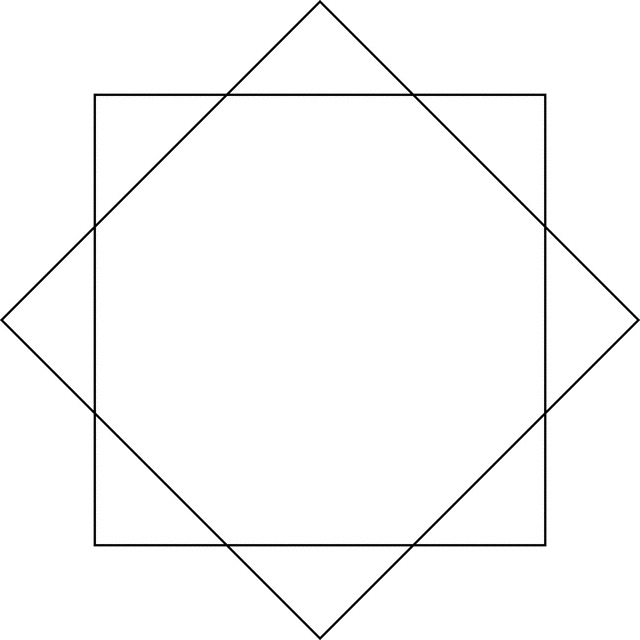
\includegraphics[width=\textwidth,height=3cm,keepaspectratio]{images/cocentric-squares}
\caption{ A pair of disks cannot have exactly 8 intersections and 10 regions  defined by them }
\label{fig:cocentric-squares}
\end{figure}

Considering squares of various radii, positions, and tilt, it is easy to show that it is impossible to map squares in general to disks while preserving point memberships. For instance, take two co-centric squares of equal size but at a 45 degree angle of each other as described in figure~\ref{fig:cocentric-squares}. This configuration produces a total of 8 intersections and 10 regions. No pair of circles in a plane can produce 10 regions and thus general squares cannot be mapped to disks. Thus we will only consider axis-parallel squares for simplicity and assume that two regions are equivalent if they are part of the same combinations of objects.

\subsection{Idea: maintaining center, choose arbitrary radius}
Counterexample drawing

\subsection{Configuration of all \texorpdfstring{$k$}{k}-depth intersections of disks for \texorpdfstring{$k=0,1,2$}{k=0,1,2}}
In an effort to explore the possibility of mapping squares to disks, we check the limits of the expressiveness of disk intersection regions. It is impossible to lay out $n$ circles to include all combinatorially possible regions of $depth=2$ for $n \geq 5$. This can be demonstrated by constructing a graph with vertices representing each disk and an edge connecting two vertices if the corresponding disks share a common $depth=2$ region and each have a $depth= 1$ region of their own. We name this graph \textbf{2-intersection graph}. Creating all combinatorially possible disk intersections of $depth=0,1,2$ means each vertex in the graph is connected to all other vertices -- in other words it is a complete graph. For $n \geq 5$ it is impossible to draw a planar complete graph. Thus if we can find a family of five squares with all combinatorially possible regions of $depth=0,1,2$, we can show that it is impossible to map squares to disks.

It is important to note, however, that there is also a limit to the number of $depth=2$ regions that can be created by axis-parallel rectangles, as we show below. Thus this approach is inconclusive.

\subsection{Set of points in maximum \texorpdfstring{$depth=2$}{depth=2} }
\label{section:thurston}
\begin{theorem}[Thurston’s coin-graph theorem]
Every planar graph G can be represented by a set of non-overlapping circles in the plane, one circle for each vertex, so that two vertices are adjacent in G if and only if the corresponding circles are tangent. \cite{Brightwell:doi:10.1137/0406017}
\end{theorem}
 
If no three squares have a common intersection or there are no points in regions of depth greater than 2, we can map squares to a 2-intersection graph, which is planar by lemma 6 of \cite{Pyrga:2008:NEP:1377676.1377708}. We can then map the graph to a set of tangent circles using Thurston's coin-graph theorem above. The circles have no intersections with each other but by increasing their radius by a small $\epsilon$, each pair of squares with $d=2$ intersection has a corresponding pair of disks.




\section{Mapping Disks to Squares}
If there exists a bijective mapping from disks to squares, we can take the mapping's inverse, which will be the mapping of squares to disks. We show below that there does not exist any such mapping. Note that in this direction, we do not want any new region to be created. 
% This begs the question: can we draw an arrangement of pseudo-disks/pseudo-disks/disks/disks that cannot be converted into disks/rectangles/rectangles/squares? The two approaches below explain that some configurations of circles are not represented in any configuration of axis-parallel squares.
% In this direction, it matters that no new region is created

\subsection{Counting Argument}

\begin{lemma}
\label{lem:maximal-planar}
The \textbf{maximal planar graph} of $n$ vertices has $3n-6$ edges.
\end{lemma}
\begin{proof}
A maximal planar graph has as each face a triangle, which consists of 3 vertices and 3 edges. For each face there are three edges, but each edge is counted twice by the two incident faces. So $F=\frac{2E}{3}$. In Euler's formula $V-E+F=2$, substitute $F=\frac{2E}{3}$ and solve to get $V=3E-6$. 
\end{proof}

The following is an incomplete counting argument that it is impossible to map disks to squares.
 By lemma 6 of \cite{Pyrga:2008:NEP:1377676.1377708}, we can represent a set of disks and their $depth=2$ intersections as a 2-intersection graph. The maximal planar graph of $n$ vertices has $3n-6$ edges by lemma \ref{lem:maximal-planar}. Then a set of $n$ disks has at most $3n-6$ $depth=2$ intersections. % it is less than 3n-6 for sure but is the lemma bidirectional? can we say that n disks can actually have 3n-6 depth=2 regions?
Starting with a single $depth=2$ intersection between two squares, we can greedily acquire two new regions of $depth=2$ every time we add a new square, as demonstrated in figure \ref{fig:depth-2-square-greedy}. So the total number of $depth=2$ regions is at least $2n-3$.
Since $3n-6 > 2n-3$ for all $n > 3$, a family of 4 or more disks has regions represented that are not reproducible with a family of equal number of axis-parallel squares.


\begin{figure}[ht]
    \centering
	\begin{minipage}[b]{.45\textwidth}
	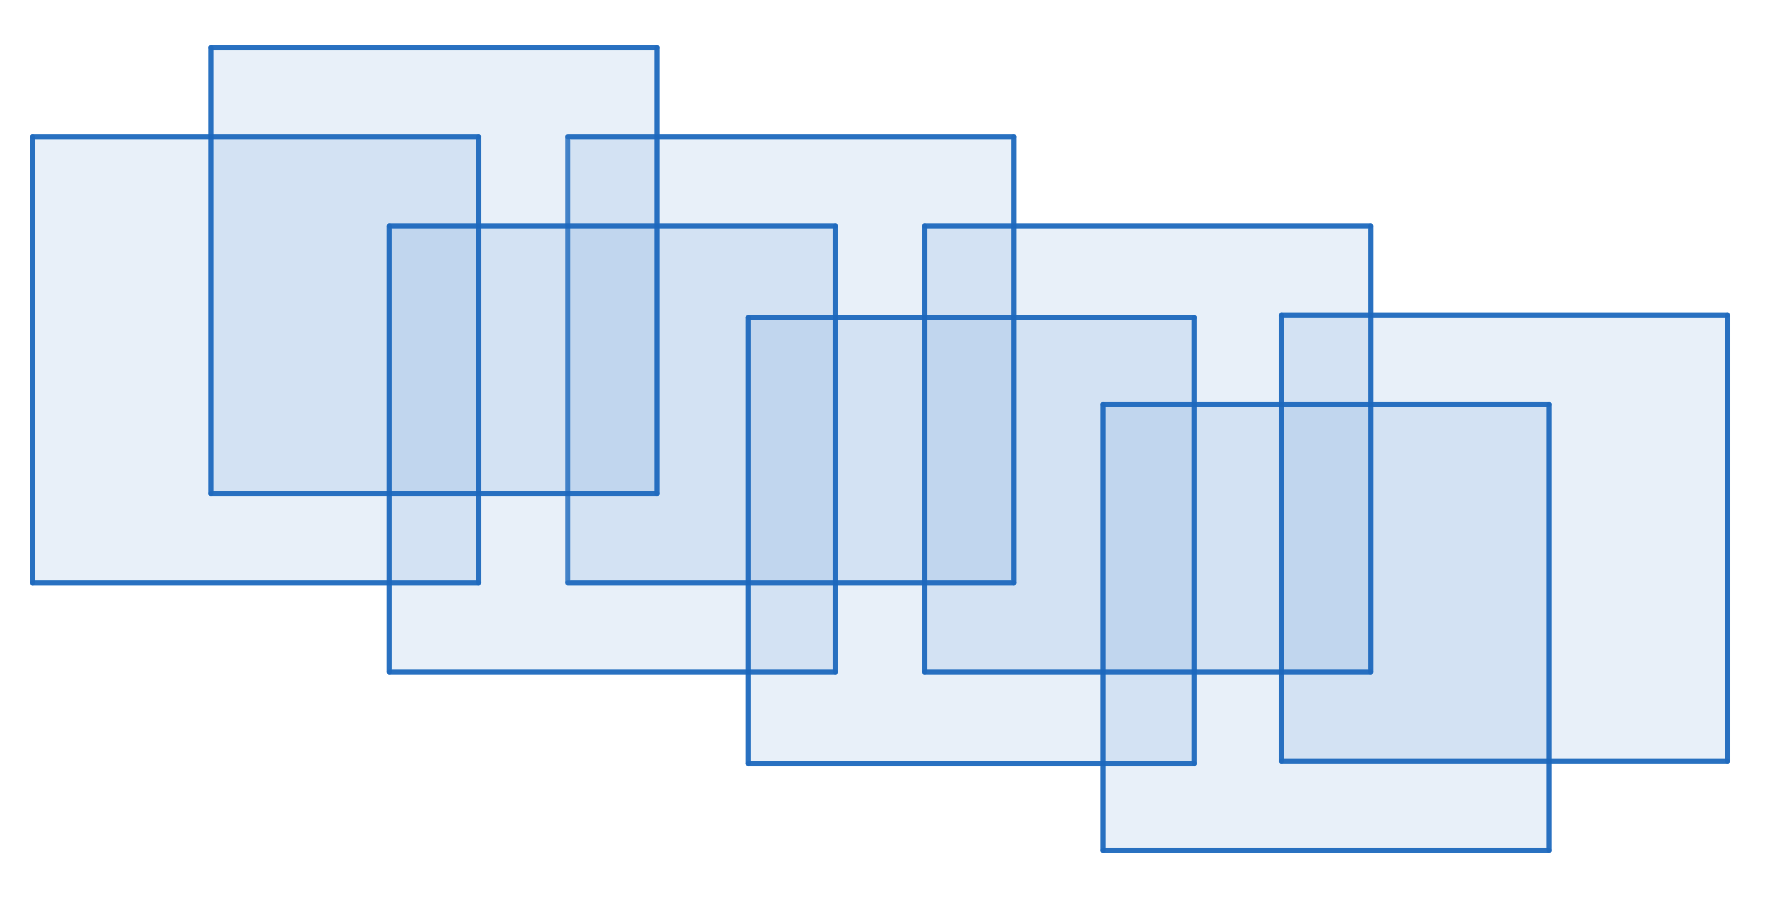
\includegraphics[width=\textwidth]{images/depth-2-square-greedy.png}
    \caption{Greedy method of obtaining $2n-3$ regions of $d=2$}
    \label{fig:depth-2-square-greedy}
	\end{minipage}
	\hfill
    \begin{minipage}[b]{.5\textwidth}
    \subfloat[]{\includegraphics[width=.48\textwidth]{k4-circles-zoomed}}
    \subfloat[]{\includegraphics[width=.48\textwidth]{k4-squares}}
    \caption{Regions in this configuration of four disks are not reproducible with four squares}
    \label{fig:k4-circles-squares}
    \end{minipage}
    
\end{figure}

This argument is an incomplete because  lemma 6 of \cite{Pyrga:2008:NEP:1377676.1377708} is not biconditional. We do not know whether $3n-6$ intersection regions of $d=2$ can be achieved with any number of disks. The inverse of the statement might be approached using a variation of the circle packing theorem. Also, we do not know whether there can be more than $2n-3$ regions of $d=2$ for any arbitrary $n$.

\subsection{Counterexample Using Three Disks and Three Rectangles}
\label{section:three-rectangles}
Multiple ($n\geq3$) circles sharing one intersection point.
related to the above. With 3 circles that intersect with common intersections for any pair but none for the triple, it's impossible to draw this with a square without creating new regions.

Given three disk, each pair can intersect with each other without a common intersection of all three. With three axis-parallel rectangles, however, if each pair intersect with each other, there is always a common interaction of all three.

\subsection{Counterexample Using Four Disks and Four Rectangles}
We prove that squares cannot generalize circles by counterexample. A set of four disks that has $K_4$ as its 2-intersection graph cannot be represented with four rectangles. Of the combinatorially describable $\binom{4}{1}$ regions of $d=1$ and $\binom{4}{2}$ regions of $d=2$, there will always be a $d=1$ or $d=2$ intersection region that is not represented.

\begin{theorem}
Given 4 axis-parallel, 2-admissible rectangles, there exist a $depth=1$ or $depth=2$ intersection region that is not attainable.
\end{theorem}
\begin{proof}
Given 3 rectangles, the following are true.
\begin{enumerate}
\item Depth=3 region is a rectangle because the intersection of any two rectangles is always a rectangle. 
\item Since the boundary of the depth=3 region is a subset of the boundaries of the rectangles, at least 2 extensions should exist in each of horizontal and vertical directions (this is true regardless of the rectangles' positions - piercing/contained/etc.)
\item The two regions on either side of any boundary must have the difference in depth of exactly 1. 
\item By (3), the regions directly above, below, left of, and right of the depth=3 region has depth=2. 
\item By (2) and (3), Since there are at least 2 extensions in each direction that are "real," at least two corners must have depth=1. (Adjacent to the real line must be a depth=1 region. Two lines always go together, since adjacent to the depth one region are two depth=2 regions, and there must be a separating line between the depth=1 and depth=2 regions. )

\end{enumerate}
\end{proof}

\begin{lemma}
There is exactly one L-shape. (equiv to one corner has depth=2)
\end{lemma}
\begin{proof}
\begin{enumerate}
\item
Since there can be at most 3 depth=2 regions, by pigeonhole principle at least two of those are the same regions. 
\item 
Not all four depth=2 regions can be the same. If they are, the depth=3 region is a contained rectangle, meaning its depth=1 region is non-existent. We do not consider such a case since if a depth=1 region cannot be represented in a configuration of three rectangles, it will not be represented even after an additional rectangle.
\item 
For three d=2 regions to be the same, two opposite regions, \textit{WLOG} B and F, would be the same region, suppose \textit{WLOG} that regions B~F are in the interior of a rectangle and lines 1 and 6 the boundary of that rectangle. There are three possible cases (0, 1-1, 1-2) as described in figure ***********which all lead to contradictions (either piercing or contained). Thus no three can be the same region either. (explain more. add a figure.)
\item 
Thus there must be exactly two regions that are the same, and by (3), they must not be across the depth=3 region, which means they share a corner and there must be exactly one L-shape.
\end{enumerate}
\end{proof}

% Premise 1. if DNE L-shape, then each of the four depth=2 regions are separated. Then all of the corners must have depth=1.
% Premise 2. not all corners can be of depth=1 since if they are, that implies either that the rectangles are piercing or their boundaries are overlapping.
% Conclusion 1. Since some corners are more than depth=1, there must be an L-Shape.
\begin{corollary}
All regions in the center map, except for the single L-shape, diagonally neighbouring the $depth=3$ region have $depth=1$.
\end{corollary}
\begin{proof}
This follows from the previous proof. Since the single $depth=2$ L-shape and the remaining two $depth=2$ regions are disjoint, there must be $depth=1$ regions that separate them.
\end{proof}


\begin{figure}[ht]
\centering
\subfloat[The $depth=3$ region and its 8 surrounding regions \label{fig:sub:depth-center}]{\includegraphics[width=0.45\textwidth]{depth-map-center}}
\subfloat[\textit{WLOG}, possible locations of upper-left corner of fourth rectangle \label{fig:sub:depth-starting-location} ]{\includegraphics[width=0.45\textwidth]{depth-map-all}} \\
\subfloat[The only three cases with all $d=1,2,3$ regions \label{fig:sub:depth-3-cases}]{\includegraphics[width=0.7\textwidth]{depth-map-3-cases}} 
\caption{Case analysis of possible configurations of three rectangles}
\label{fig:depth-map}
\end{figure}

Now we have the exact picture of the 8 regions around the center $depth=3$ region, as depicted \textit{WLOG} in figure \ref{fig:depth-map}.  There are three general cases that have all $d=1,2,3$ regions represented. 

In order to generate the three new $d=2$ regions, the fourth rectangle must intersect all three $d=1$ regions. In order to conserve the three pre-existing $d=2$ regions, the fourth rectangle must not completely contain any one of them. 





\section{Reducing Counterexamples of Unrepresented Half-Spaces}
Hypothetically, computers can check all combinations (with 5 squares there are already 16 possible regions) to claim that a certain configurations of squares and points can topologically map or not. If it's not possible to map a certain configuration of squares and points, there would be a logical inconsistency in the system somewhere. Instead of checking all combinations, it would be ideal to check a smaller number of combinations  to conclude that a mapping is impossible. Thus it would be helpful to show that any counterexample can be reduced to a small counterexample, say of size two or three squares.

We approach this problem from a lower level, using pseudo-lines in $\mathbb{R}^2$ instead of half-spaces in $\mathbb{R}^3$. A matrix is used to abstractly describe the configuration of the pseudo-lines and points on the plane. Each row of the matrix represents a pseudo-line $c_i$ and each column represents a point $p_j$. 
\begin{equation*}
M_{ij} =\begin{cases}
            	+1 & \text{if $c_i$ is above $p_j$,} \\
                -1 & \text{if $c_i$ is below $p_j$}
            \end{cases}
\end{equation*}
Without loss of generality, choose the following as the ``forbidden pattern:" 
\begin{equation}
\begin{bmatrix}
    +1 & -1 \\
    -1 & +1 
\end{bmatrix}
\end{equation}
The above pattern appears whenever an inconsistency exists in a system of two or more curves and three or more points:
\begin{align*}
\begin{bmatrix}
    +1 & -1 & +1 \\
    -1 & +1 & -1
\end{bmatrix} \text{ or }\ 
\begin{bmatrix}
    -1 & +1 & -1  \\
    +1 & -1 & +1
\end{bmatrix}
\end{align*}
The two cases above cannot exist since pseudo-lines can only intersect each other at most once but these configurations necessarily mean that there are at least two intersections between the two curves. 

\subsection{Reducing to smallest counterexample}
Define a graph of vertices representing the pseudo-lines and a directed edge from $c_i$ to $c_j$ if for $a<b$ the following ``intersection" pattern exists:

\begin{center}
% \centering
\begin{tabular}{c|c c c c c }
                     & $p_a$   & \dots  & $p_b$      \\ \hline
$c_i$                  &  -1   &        & +1       \\
\vdots               &       &        &          \\
$c_j$                  &  +1   &        & -1  \\
\end{tabular}
\end{center}

The existence of this pattern means that $c_i$ and $c_j$ intersect between the two points $p_a$ and $p_b$. Here we show that if there is a cycle of size $n$, it will inevitably admit the forbidden pattern. Suppose there exists a cycle of size $n$ without any forbidden patterns:

\begin{center}
\begin{tabular}{c|c c c c c }
                 & \dots& 2n-3  & 2n-2  & 2n-1  & 2n \\ \hline
$c_1$              &      &       &       &  +1   &  -1   \\
$\vdots$           &      &       &       &       &    \\
$c_{n-1}$          &      &  -1   &   +1  &       &    \\
$c_{n}$            &      &  +1   &   -1  &  -1   &  +1 \\
\end{tabular}
\end{center}

Since this matrix does not have any forbidden patterns, $c_1$ must be above $p_{2n-3}$.
\begin{center}

\begin{tabular}{c|c c c c c }
            & \dots & 2n-3  & 2n-2  & 2n-1  & 2n \\ \hline
$c_1$         &       & \cellcolor[HTML]{FFFFC7}{\color{blue}+1}  &    & \cellcolor[HTML]{FFFFC7} +1   & -1    \\
$\vdots$      &       &       &       &       &    \\
$c_{n-1}$     &       &  -1   &  +1   &       &    \\
$c_{n}$       &       & \cellcolor[HTML]{FFFFC7} +1               & -1 & \cellcolor[HTML]{FFFFC7}  -1  &  +1 \\
\end{tabular}
\end{center}

Since this matrix does not have any forbidden patterns, $c_{n-1}$ must be above $p_{2n}$.

\begin{center}
\begin{tabular}{c|c c c c c }
                    & \dots & 2n-3 & 2n-2 & 2n-1 & 2n \\ \hline
$c_1$                 &       &\cellcolor[HTML]{FFFFC7} +1       &          &  +1    &\cellcolor[HTML]{FFFFC7} -1    \\
$\vdots$          &            &         &          &          &    \\
$c_{n-1}$   &            &  \cellcolor[HTML]{FFFFC7}-1    &  +1    &          &  \cellcolor[HTML]{FFFFC7} {\color{blue}-1} \\
$c_{n}$      &             &  +1   &   -1  &  -1    &  +1 \\
\end{tabular}
\end{center}

However, we have a contradiction since there exists a forbidden pattern:

\begin{center}
\begin{tabular}{c|c c c c c}
                      & \dots & 2n-3 & 2n-2 & 2n-1 & 2n \\ \hline
$c_1$              &            & +1       &          &  +1    & -1    \\
$\vdots$          &            &         &          &          &    \\
$c_{n-1}$   &            &  -1    & \cellcolor[HTML]{CB0000} +1    &          &  \cellcolor[HTML]{CB0000} -1 \\
$c_{n}$      &             &  +1   &  \cellcolor[HTML]{CB0000} -1  &  -1    & \cellcolor[HTML]{CB0000} +1 \\
\end{tabular}
\end{center}

Thus if in a configuration of pseudo-disks there exists a cycle of size $\geq 3$, it must admit a small counterexample that is namely the forbidden pattern. This means that all that is needed to show that a system of pseudo-lines and points is inconsistent is to look for a single forbidden pattern.

\subsection{Permutable curves}

Define $-1 < +1$ and lexicographically sort all of the rows. If the forbidden pattern exists in the the sorted matrix, we know that there must be a cycle of size $\geq 3$.

\subsection{Permutable curves and points}

\subsection{Using Helly}

\section{Computational approaches using Convex Optimization software}
We attempt using a convex optimization problem solver software in order to find a counterexample for a large number of points and squares. 

If for each execution the software finds a viable mapping from finite squares and points to half-spaces, it is inconclusive and does not imply anything. However, if the software concludes that there exist no mapping for a certain configuration of squares and points, such a configuration is the counterexample demonstrating that squares cannot be lifted to half-spaces in general. In either case, it could provide us with more insight on cases that are too big to be imaginable.

\subsection{Mapping a set of squares to a set of half-spaces (Incorrect) }
 The idea is to create variables that represent points and half-spaces in $\mathbb{R}^3$. If for each execution the software finds a viable mapping from finite squares and points to half-spaces, it is inconclusive and does not imply anything. However, if the software concludes that there exist no mapping for a certain configuration of squares and points, such a configuration is a counterexample demonstrating that squares cannot be lifted to half-spaces in general. In either case, it could provide us with more insight on cases that are too big to be imaginable.

Below is the setup of the convex optimization problem. If a mapping from a given set of squares to some set of half-spaces exists, the solver will find it.

\begin{enumerate}
\item Randomly sample set of $m$ points in $\mathbb{R}^2$ \begin{equation*}
				P_i = (\alpha, \beta)
\end{equation*}
\item Randomly sample $n \times 4$ values that define $n$ axis-parallel squares \begin{equation*}
				S_j=(left,right,top,bottom)
			\end{equation*}
\item For each $i,j$ pair, save the binary membership flag \begin{equation*}
M_{ij} =\begin{cases}
            	1 & \text{if $P_i$ inside $S_j$,} \\
                -1 & \text{otherwise}
            \end{cases}
\end{equation*}
\item Create $m \times 3$ variables representing points in $\mathbb{R}^3 $ \begin{equation*}
			Q_i = (x_i,y_i,z_i, 1)
\end{equation*}
\item Create $n \times 3$ variables representing half-spaces in $\mathbb{R}^3 $ \begin{equation*}
				H_j = (a_j,b_j,c_j, 1)
\end{equation*}
\item Create $m \times n$ constraints \begin{equation*}
			M_{ij}(Q_i \cdot H_j) > 0
\end{equation*}
\item Set the objective function as simple expression, say 1, and solve.


\end{enumerate}
This approach was found to be incorrect because our constraints are in the form of a dot product of two variable vectors, which is a rational inequality and thus not a convex problem.


\subsection{Mapping a set of squares to a set of disks}

We want to see whether there are some intersection regions of squares (square-cells) that cannot be expressed as intersection regions of circles (circle-cells). To do that, we represent each square-cell by the indices of the squares that the square-cell is a subset of. Each line after the first in input.txt are the indices of the squares that the square-cell consists of. 

\begin{figure}[ht]
\subfloat[input]{\includegraphics[width = 0.33\textwidth]{convex-opt-square}}
\subfloat[possible solution]{\includegraphics[width = 0.33\textwidth]{convex-opt-sol-1}}
\subfloat[another possible solution]{\includegraphics[width = 0.33\textwidth]{convex-opt-sol-2}}
\caption{
% examples of input/output
}
\label{fig:convex-opt}
\end{figure}

Assuming there exists a solution that satisfies the demands, each corresponding circle-cell will have a point that is less than 1 metric unit away from the center of each circle that makes up the circle-cell:
% d((y_i ) ⃗, (x_j ) ⃗  )<1

If a square xj does not comprise a square-cell, for all points (we will only constrain one point) yi in the circle-cell,
% d((y_i ) ⃗, (x_j ) ⃗  )>1


The first line (n,m) is number of squares and number of demands/regions that we will make.
Matrix M of demands is 

% M_ij∗d((y_i ), (x_j ) ⃗  )<M_ ij

Number of variables: 2*(n+m)
Number of constraints: n*m

If using gradient descent: $L = \sigma(d(a,b)-1)$ if section a in circle b else $\sigma(1-d(a,b))$ using sigmoid function


\subsection{Justification}
If there exists a point in a subsection of a circle, then the distance from the point to the center of the circle is less than 1 (unit radius). If the same subsection is not a subsection of another circle, the point must be farther away from the center of the second circle.

\subsection{Relation to VC Dimension}

\subsection{Spectral Clustering}

\section{Lifting Paths of a Graph}
We have demonstrated above in subsection~\ref{section:thurston} how to map a planar graph to disks with maximum $d=2$. Lifting a vertex $P_1$ on a 2-intersection graph is  equivalent to lifting circles.

Lifting two adjacent vertices $P_2$ has implications regarding intersection regions. We define two vertices representing pseudo-disks are adjacent if there is a point in the intersection region. The edge represents the intersection region. Lifting two adjacent vertices means we lift the edge connecting them as well.

Lifting a face $C_3$ of three vertices has implications regarding axis-parallel rectangles. We showed in section~\ref{section:three-rectangles} that if every pair in a set of three such rectangles intersect with each other, there must be a common intersection of all three. Thus $C_3$ represents three rectangles that have a common intersection.

We do not see a clear implication of lifting a path $P_3$ of $length=3$ regarding pseudo-disks, however, we still show that it is possible to lift a set of non-crossing $P_3$ in star graphs and tree graphs.


\subsection{Lifting vertices, edges, and faces}

We show that it is possible to lift vertices, edges, and triangular faces in any position in a planar graph with the help of Steinitz's Theorem stated below. 

\begin{theorem}[Steinitz's Theorem \cite{weisstein}]
Every 3-connected planar graph can be realized as a convex polyhedron. 
\end{theorem}

Take any planar graph of size $n \geq 4$ and triangulate it so that it becomes the maximal planar graph. The maximal planar graph is at least 3-connected so Steinitz's Theorem is applied to it, lifting the graph to a 3D polyhedron. Note that the original vertices, edges, and triangular faces are conserved in the polyhedron. Take the half-space defined by a point and the normal vector on each object. Translate it in the opposite direction of the vector by a small distance $\epsilon$. The resulting half-space separates the given object from the rest of the graph.

\subsection{Lifting paths of \texorpdfstring{$length=3$}{length=3}}
In order to make a more general statement about triangular faces, we consider any set of $length=3$ paths, \textit{i.e.} triples, that is in a planar graph. It is not clear how to generalize lifting triangular faces into $length=3$ paths using the polyhedron transformation described above. For simplicity at this stage, we disregard sets in which a pair of triples cross each other through the middle vertex.

\paragraph{Redrawing of graph} One graph that never has any crossing triples is a binary tree. A binary tree can be redrawn according to the following recursive construction in order to lift any number of paths in the graph.
\begin{enumerate}
\item Start from the root node and base length 1 as distance to its children.
\item If the current node has a parent, take a fraction $r\leq 1$, say half, of the distance between the parent and the current node as its distance to its children nodes.
\item Depending on the value of $r$, take $\theta$, say $\frac{\pi}{2}$, as the angle between the edges to the current node's two children.
\end{enumerate}

\paragraph{Lifting} The following is the lifting step.
\begin{enumerate}
\item There exists a unique circle $C_i$ passing through the parent and two children of each node $v_i$.
\item Every triple as well as an extra node is inside the circle defined by the middle node.
\item To exclude the extra node, define a new disk by maintaining the two leaves of the triple on the boundary of the disk but translating the center towards the midpoint of the two leaf nodes by a small $\epsilon$.
\item Repeat this for all given triples.
\item Using the mapping described in section~\ref{section:disk-lifting}, each triple but no other node is lifted to a half-space.
\end{enumerate}

\begin{figure}[ht]
\centering

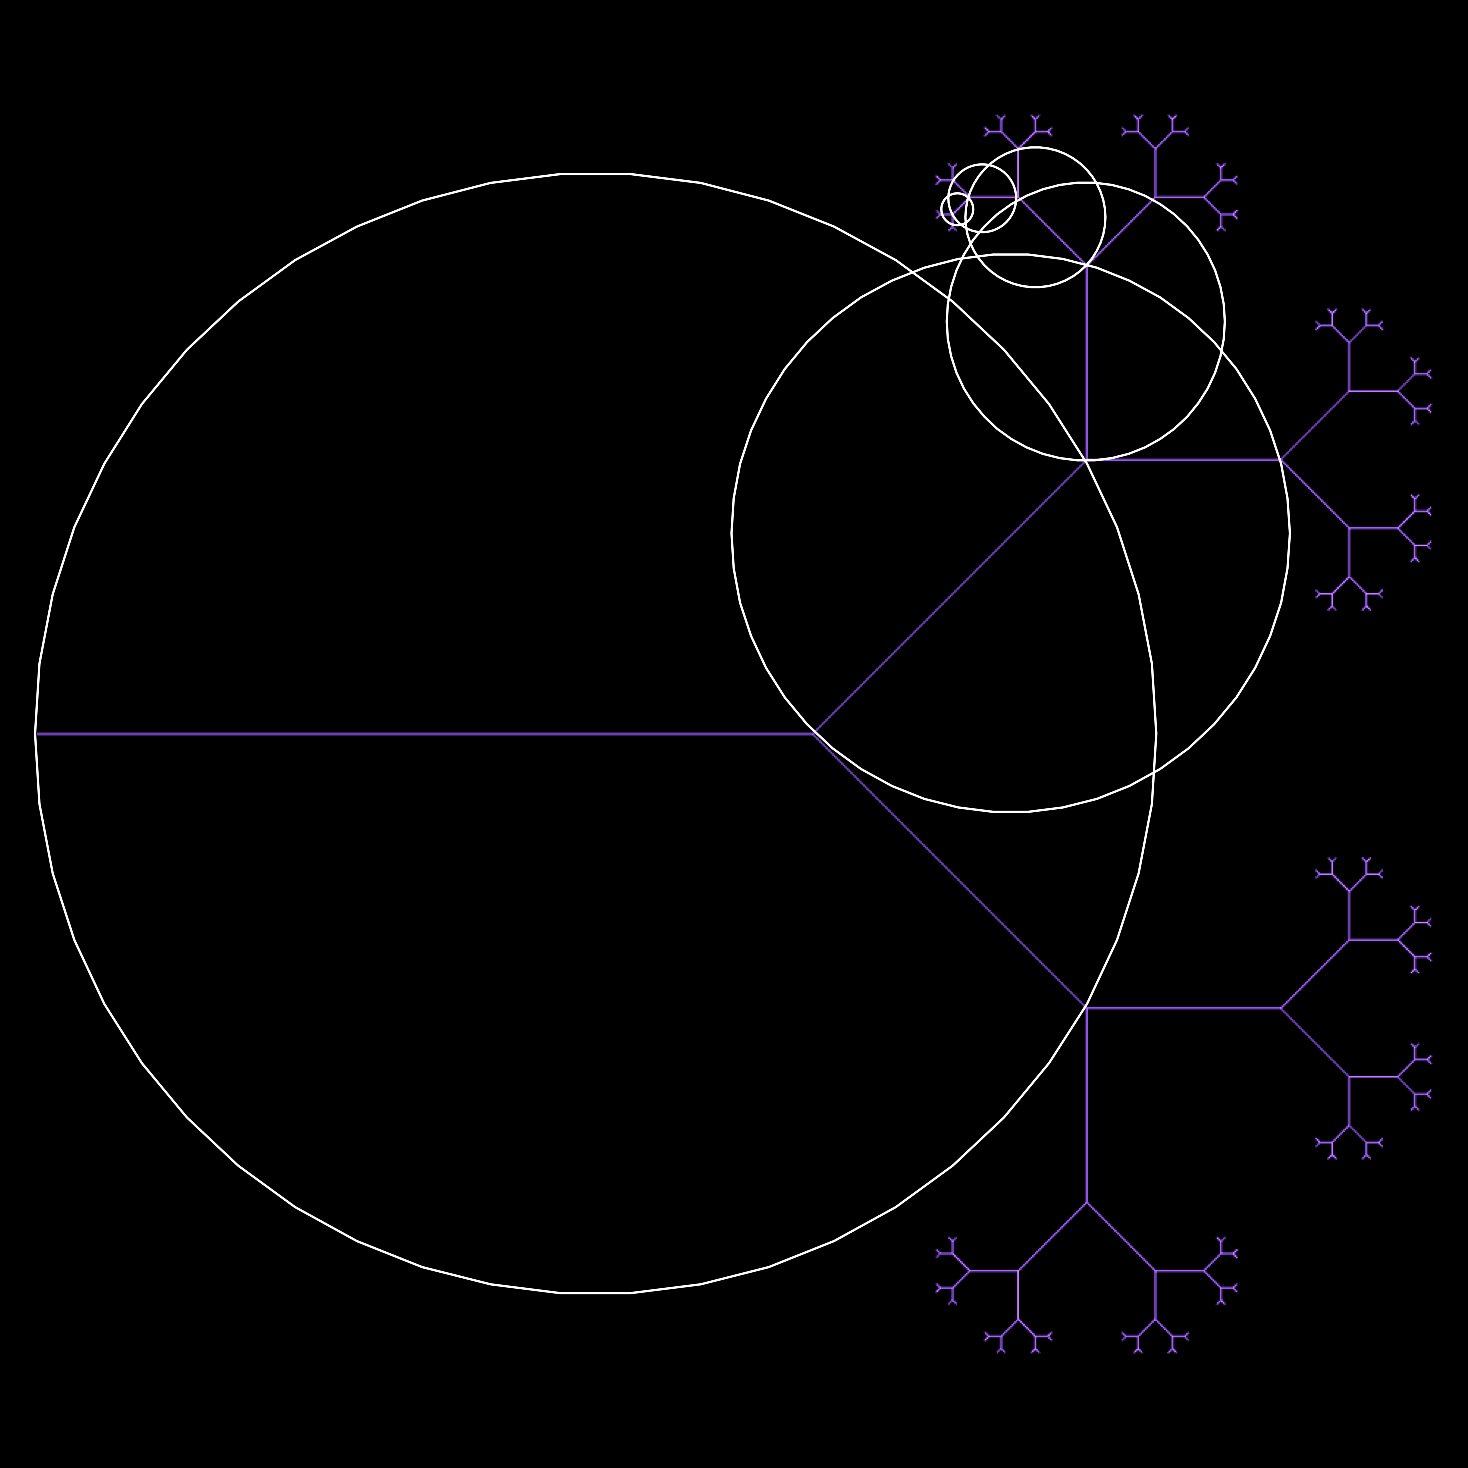
\includegraphics[width=0.5\textwidth]{images/binary-tree-with-circles}
\caption{Any $P_3$ in a binary tree $G$ is separable from $G\backslash P_3$ by a circle}
\end{figure}


We require the distance to decrease exponentially so that we can generalize binary trees of arbitrary heights. The angle $\theta$ needs to be small in order to prevent the two descendant branches from curving back into the circle in which the parent node exists as well as into each other.

\begin{theorem}
In a drawing of a binary tree with $r=\frac{1}{2}$, $\theta=\frac{\pi}{2}$, the subtrees with the two children nodes of node $v_i$ as roots do not intersect the unique circle $C_i$ passing through the parent and two children of $v_i$.
\end{theorem}
\begin{proof}

\end{proof}

\begin{theorem}
In a drawing of a binary tree with $r=\frac{1}{2}$, $\theta=\frac{\pi}{2}$, the subtrees with the two children nodes of node $v_i$ as roots do not intersect each other.
\end{theorem}
\begin{proof}

\end{proof}

generalize for k-ary tree

proof by construction of star
corollary: star

\newpage
\section{Appendix: Definitions}
\begin{enumerate}
\item A geometric shape is \textbf{axis-parallel} if it is parallel or aligned with a coordinate 
\item axis.
\item The \textbf{depth} of a region formed by the intersection of multiple Jordan curves is the number of Jordan curves that the region is inside of.
\item A \textbf{half-space} in $\mathbb{R}^3$ is either of the two parts separated by a plane. In general, a half-space is either of the two parts divided by a hyperplane in $\mathbb{R}^k$.
\item \textbf{Helly's theorem} for the Euclidean plane states that if a family of convex sets has a nonempty intersection for every triple of sets, then the whole family has a nonempty intersection. (Wikipedia)
\item A \textbf{Jordan Curve} is a curve in a plane that is topologically equivalent to a disk - simple and closed.
\item A family of \textbf{k-admissible} regions (for k even) are regions bound by Jordan curves that if for any two $s_1$, $s_2$ of the regions, the Jordan curves bounding them cross (two Jordan curves cross when at a certain point a curve passes from one side of another curve to the other) in l ≤ k points, (for some even l), and both $s1\backslash s2$ and $s2\backslash s1$ are connected regions. \cite{Pyrga:2008:NEP:1377676.1377708}
\item \textbf{Lifting} is mapping a geometric object in one dimension to a higher dimension.
\item A simple graph is called \textbf{maximal planar} if it is planar but adding any edge (on the given vertex set) would destroy that property. All faces (including the outer one) are then bounded by three edges. (Wikipedia)
\item \textbf{Membership} of a point and a region is a binary flag that signifies whether the point is inside the region or not.
\item A Jordan curve $C$ \textbf{pierces} another Jordan curve $D$ if all curves in the interior of $D$ connecting any two points inside $D$ must cross $C$ at least twice.
\item \textbf{Pseudo-disks}, or 2-admissible regions, are a set of regions defined by the interior of Jordan curves in $\mathbb{R}^2$ in which any pair of the Jordan curves intersect at maximum two places and do not pierce one another. This property is derived from disks in $\mathbb{R}^2$.
\item \textbf{Pseudo-lines} are a set of curves that intersect one another at most once. This property derives from that of lines.
\item A \textbf{2-intersection graph} is a graph with vertices representing each pseudo-disk and an edge between two vertices if the corresponding pseudo-disks share a common $depth=2$ region and each have a $depth=1$ region of their own.

\end{enumerate}


\newpage
\renewcommand\refname{References}
\bibliography{references}
% The IEEE bibliography style is NOT rBibliography listing all cited references.
% Feel free to use whatever style you prefer
\bibliographystyle{IEEEtran}

\end{document}

